\chapter{Experimental Results}

All experiments in this thesis used a set of standard conditions.  First, the length and width of each puzzle piece was set to 28~pixels per the standard established by~\cite{cho2010} and subsequently used by~\cite{pomeranz2011, gallagher2012, sholomon2013, paikin2015}. What is more, the Mixed-Bag Solver was passed no information concerning piece location nor rotation.  Furthermore, no information concerning the size of the dimensions or number of pieces in each ground-truth image is provided to the solver.  Concerning the number of input puzzles, Paikin~\& Tal's algorithm requires this information; as such, all runs of their algorithm were supplied this, meaning their algorithm is by definition solving a simpler problem.  Despite that, the Mixed-Bag Solver still generally outperforms their algorithm.

To compare the performance of the Mixed-Bag Solver and Paikin~\& Tal's algorithm on multiple images, this thesis used Pomeranz~\textit{et al.}'s dataset that contains 20 images, each of which 805 pieces.  In each test, a specified number of images (ranging from 2 were selected, without replacement from the pool of 20 images.  The outputs generated by the two algorithms were then compared.  Table~\ref{tab:numberSolverIterations} shows the number of times the solvers were run with the specified number of puzzles as the input. As explained in Section~\ref{sec:assemblerTimeComplexity}, the execution time of Paikin~\& Tal's assembler can grow cubicly, in particular if Best Buddy Density is low.  As such, the solver was performed fewer times as the number of input puzzles increased.

\begin{table}[tb]
\begin{center}
\begin{tabular}{ |c||c|c|c|c| } 
 \Xhline{1pt}
 \# Puzzles    &  2 &  3 & 4 & 5 \\ 
\hline \hline
 \# Iterations & 55 & 25 & 8 & 5 \\ 
 \Xhline{1pt}
\end{tabular}
\end{center}
\caption{Number of Solver Iterations for Each Puzzle Input Count}\label{tab:numberSolverIterations}
\end{table}

\section{Accuracy Determining the Number of Input Puzzles}

For the Mixed-Bag Solver to provide meaningful outputs, it must be able to identify the number of ground-truth inputs provided to the solver.  The test dataset used to measure the solver's performance in this area was published by Pomeranz~\textit{et al.} in~\cite{pomeranzBenchmarkImages}; the dataset consists of 20~images, each of which has 805~pieces.

The next subsection discusses the solver's performance when provided only a single image.  This is separated from the more general discussion as the algorithm's performance on a single image marks the ceiling of its performance.  The algorithm's performance when solving two to five puzzles is discussed in a separate subsection.

\subsection{Single Puzzle Solving}

The Mixed-Bag solver was able to correctly identify the single ground-truth image for  17~out of the 20~images (i.e., 85\% accuracy).  For the remaining 3~images, the solver estimated that there were 2~images, meaning the error was at most only a single puzzle.  Appendix~\ref{chap:incorreclyClassifiedSingleImages} shows the ground-truth image as well as the outputs from Paikin~\& Tal's algorithm as well as this thesis' Mixed-Bag Solver.  

The Mixed-Bag Solver struggled to correctly identify the number of inputs when the image has large areas with little variation (e.g., a blue sky, smooth water, etc.). Two example images from the test dataset are shown in Figure~\ref{fig:pomeranzBestBuddiesVisualizations} shows two images in the Pomeranz~\textit{et al.}.  The Mixed-Bag Solver was able to perfectly reconstruct image~(a); in contrast, the Mixed-Bag Solver thought the pieces from image~(b) came from two separate puzzles.\footnote{Appendix~\ref{chap:incorreclyClassifiedSingleImages} shows the three images that were incorrectly identified by the Mixed-Bag Solver as well as the solver outputs generated.} The best buddy visualizations in Figure~\ref{fig:pomeranzBestBuddiesVisualizations} shows two images in the Pomeranz~\textit{et al.} show that image~(a) had a significantly higher best buddy density as well as much fewer interior non-adjacent best buddies.  It is these two factors the contributed the most to the Mixed-Bag Solver being unable to determine the number of input images for the three puzzles. 

\begin{figure}[tb]
\centering
  \begin{tabular}{ >{\centering\arraybackslash}m{0.47\textwidth} >{\centering\arraybackslash}m{0.47\textwidth} }

	\fbox{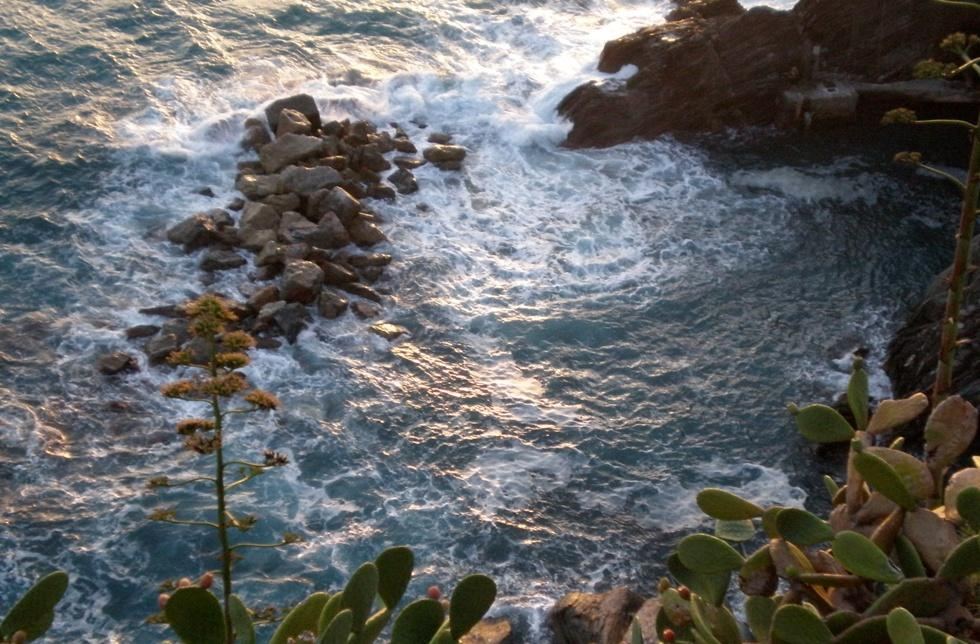
\includegraphics[scale=0.18]{./images/single_puzzle/pomeranz_805_14.jpg}} & \fbox{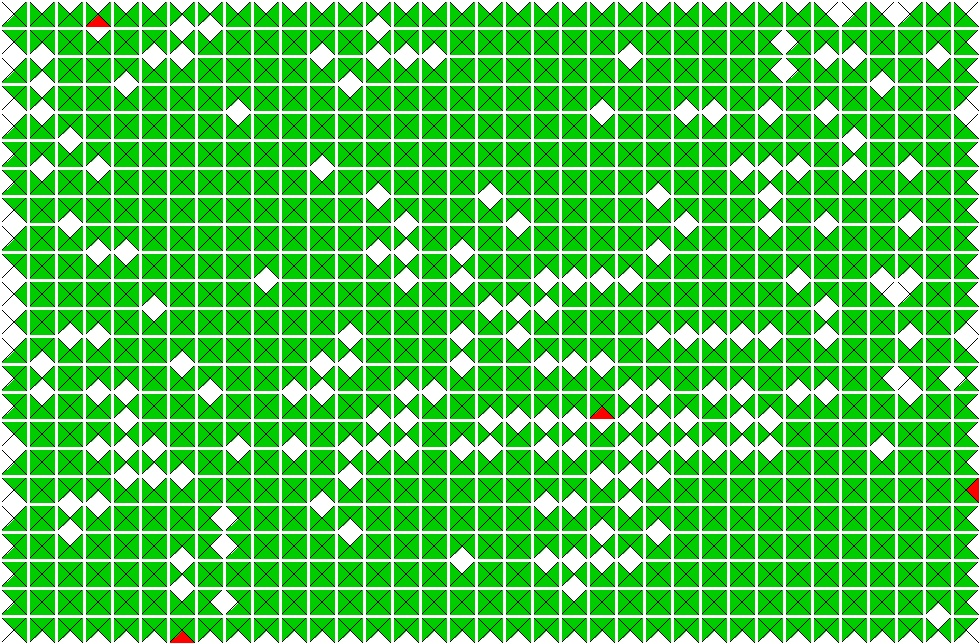
\includegraphics[scale=0.18]{./images/single_puzzle/best_buddies_pomeranz_805_14.jpg}} \\~\\
	Ground-Truth Image~(a) & Best Buddy Visualization of Image~(a) 
\\~\\
	\fbox{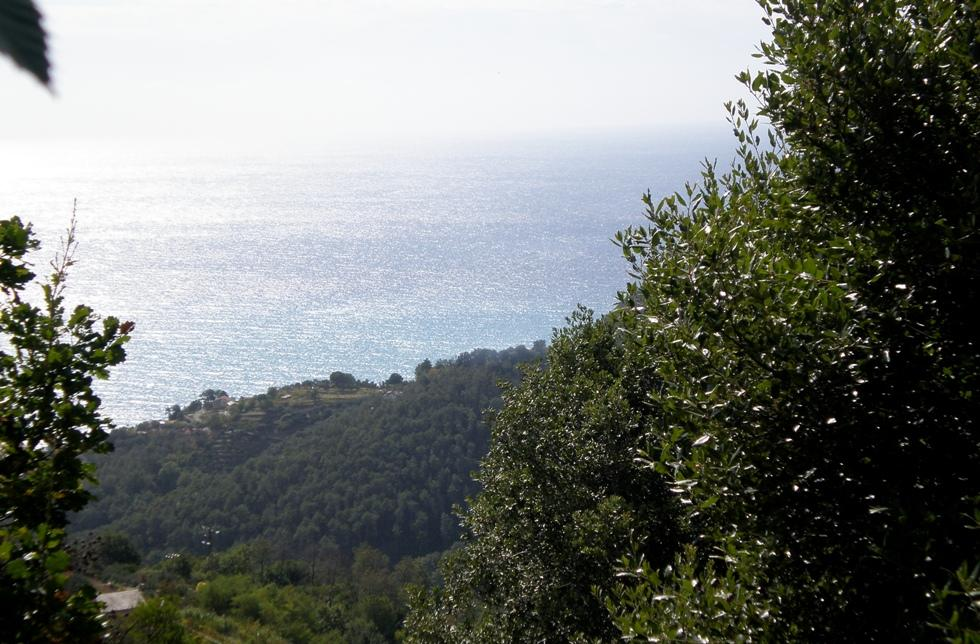
\includegraphics[scale=0.18]{./images/single_puzzle/pomeranz_805_12.jpg}} & \fbox{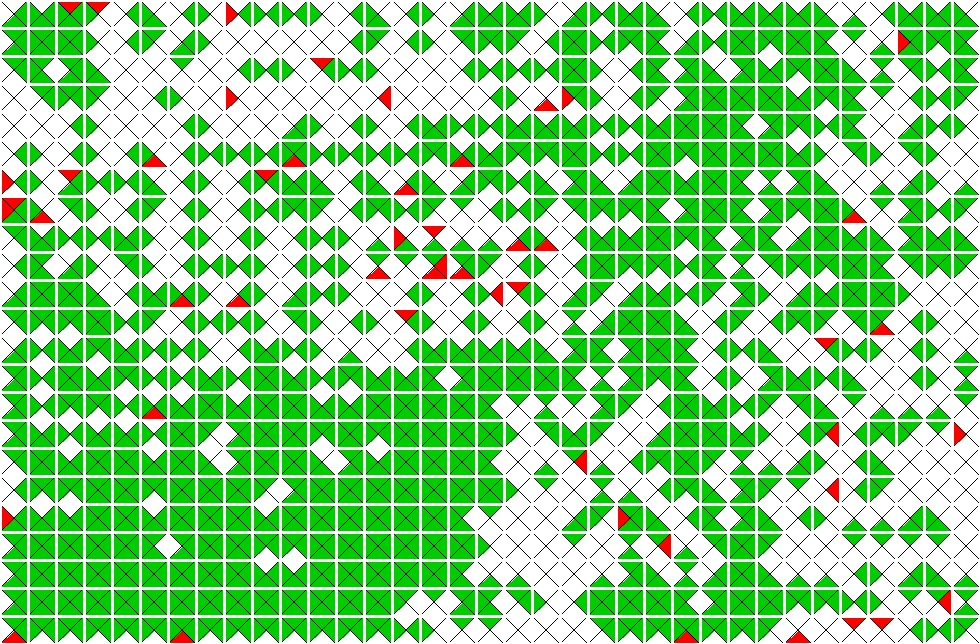
\includegraphics[scale=0.18]{./images/single_puzzle/best_buddies_pomeranz_805_12.jpg}} \\~\\
	Ground-Truth Image~(b) & Best Buddy Visualization of Image~(b) 
  \end{tabular}
\caption{Comparison of Best Buddy Density and Interior Non-Adjacent Best Buddies for Two Images from the Pomeranz \textit{et al.} 805 Piece Dataset}
\label{fig:pomeranzBestBuddiesVisualizations}
\end{figure} 

It is important to note that the difficulty the Mixed-Bag Solver has reconstructing images with low Best Buddy Density is actually an artifact of the assembler and not the solver.  Paikin~\& Tal mentioned in~\cite{paikin2015} that their solver may yield ``unsatisfactory results'' on such images.

\subsection{Multiple Puzzle Solving}

As mentioned previously, the Mixed-Bag Solver was tested by randomly selecting a specified number of images, without replacement, from Pomeranz \textit{et al.}'s  from the 805~piece dataset.  In total, Table~\ref{tab:numberSolverIterations} shows the number of times the solver was run for each input size. Figure~\ref{fig:inputPuzzleCountErrorFrequency} illustrates the performance of the Mixed-Bag Solver in determining the number of input.  A correct estimation of the number of puzzles would represent an error of ``0'' in the figure.  Similarly, an overestimation of a single puzzle (e.g., the solver identifying four puzzles when only three were provided as an input) would represent an error of ``1.''  Across all of the experiments, the Mixed-Bag Solver never underestimated the number of input puzzles; what is more, it never overestimated the number of input puzzles by more than 3.  

\begin{figure}
\begin{center}
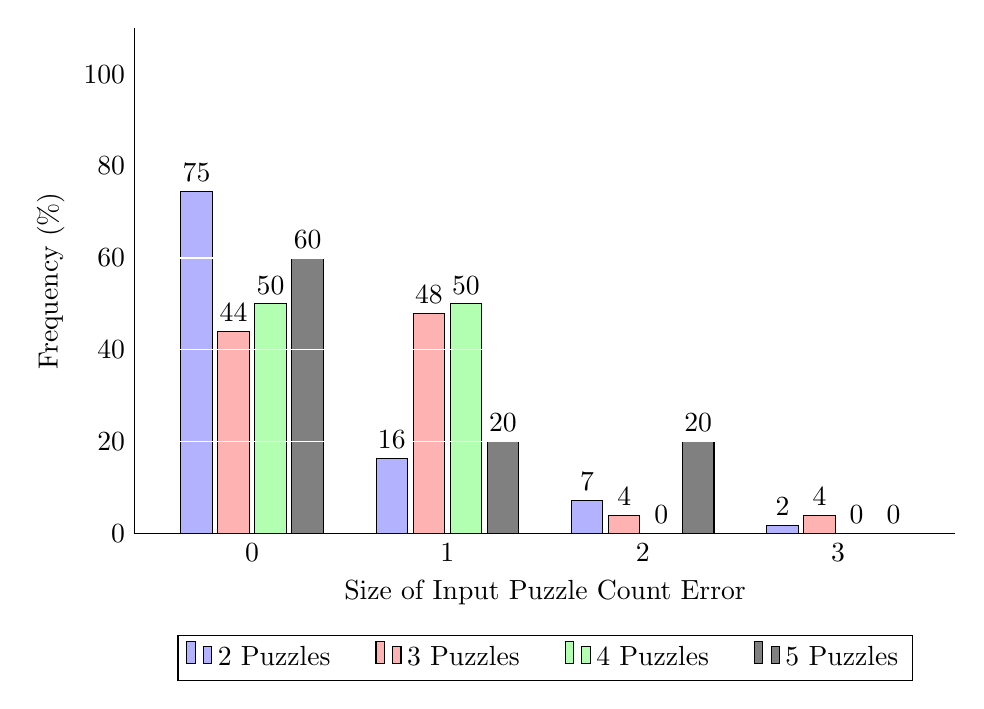
\begin{tikzpicture}
  \begin{axis}[
        ybar, axis on top,
        height=8cm, width=12cm,
        bar width=0.4cm,
        ymajorgrids, tick align=inside,
        major grid style={draw=white},
        enlarge y limits={value=.1,upper},
        ymin=0, ymax=100,
        axis x line*=bottom,
        axis y line*=left,
        y axis line style={opacity=1},
        tickwidth=0pt,
        enlarge x limits=0.2,
        legend style={
            at={(0.5,-0.2)},
            anchor=north,
            legend columns=-1,
            /tikz/every even column/.append style={column sep=0.5cm}
        },
        xlabel={Size of Input Puzzle Count Error},
        ylabel={Frequency (\%)},
        symbolic x coords={
           0, 1, 2, 3},
       xtick=data,
       nodes near coords={
        \pgfmathprintnumber[precision=0]{\pgfplotspointmeta}
       }
    ]
\addplot [fill=blue!30]
	coordinates {(0,74.5) (1,16.4)
		 (2,7.3) (3,1.8)};
\addplot [fill=red!30]
	coordinates {(0,44) (1,48)
		 (2,4) (3,4)};
\addplot [fill=green!30]
	coordinates {(0,50) (1,50)
		 (2,0) (3,0)};
\addplot 
	coordinates {(0,60) (1,20)
		 (2,20) (3,0)};
\legend{2 Puzzles, 3 Puzzles, 4 Puzzles, 5 Puzzles}
\end{axis}
\end{tikzpicture}
\end{center}
\caption{Mixed-Bag Solver's Input Puzzle Count Error Frequency}
\label{fig:inputPuzzleCountErrorFrequency}
\end{figure}

In this set of experiments, the Mixed-Bag solver correctly determined the number of input puzzles in 65\% of the tests.  Likewise, in less than 8\% of the tests did the solver overestimate the number of input puzzles by more than one.  Since the solver never underestimated the number of input puzzles, it is clearly that the solver is over-rejecting the merger of cluster and/or creating very small clusters that are too isolated to merge with the main cluster.  It is expected that the performance of the solver would be improved by reducing the minimum clustering threshold (see Section~\ref{sec:hierarchicalClustering}) as well as increasing the minimum segment size (see Section~\ref{sec:segmentPuzzle}). 

\section{Comparison of Solver Output Quality}


\begin{table}[tb]
\begin{center}
\begin{tabular}{ c||c|c|c||c|c|c||c|c|c } 
 \toprule
 \# of & \multicolumn{3}{c||}{Average SEDAS} & \multicolumn{3}{c||}{Average ENAS} & \multicolumn{3}{c}{Perfect Reconstruction} \\ \cline{2-10}
 Puzzle & MBS$\dagger$ & MBS$\ddagger$ & Paikin & MBS$\dagger$ & MBS$\ddagger$ & Paikin & MBS$\dagger$ & MBS$\ddagger$ & Paikin \\ 
 \hline \hline
 
	2 & 0.850 & 0.757 & 0.321 & 0.933 & 0.874 & 0.462 & 29.3\% & 23.6\% & 5.5\% \\ \hline
 
	3 & 0.953 & 0.800 & 0.203 & 0.955 & 0.869 & 0.364 & 18.5\% & 18.8\% & 1.4\% \\ \hline
  
	4 & 0.881 & 0.778 & 0.109 & 0.920 & 0.862 & 0.260 & 25.0\% & 15.6\% & 0\% \\ \hline
  
	5 & 0.793 & 0.828 & 0.099 & 0.868 & 0.877 & 0.204 & 20.0\% & 24\% & 0\% \\ 
 \bottomrule
\end{tabular}
\end{center}
\caption{Comparison of Mixed-Bag and Paikin~\& Tal Solvers Performance on Multiple Input Puzzles}\label{tab:tableSolverPerformanceComparison}
\end{table}

\begin{figure}[tb]
\begin{tabular}{ >{\centering\arraybackslash}m{0.95\textwidth}} 
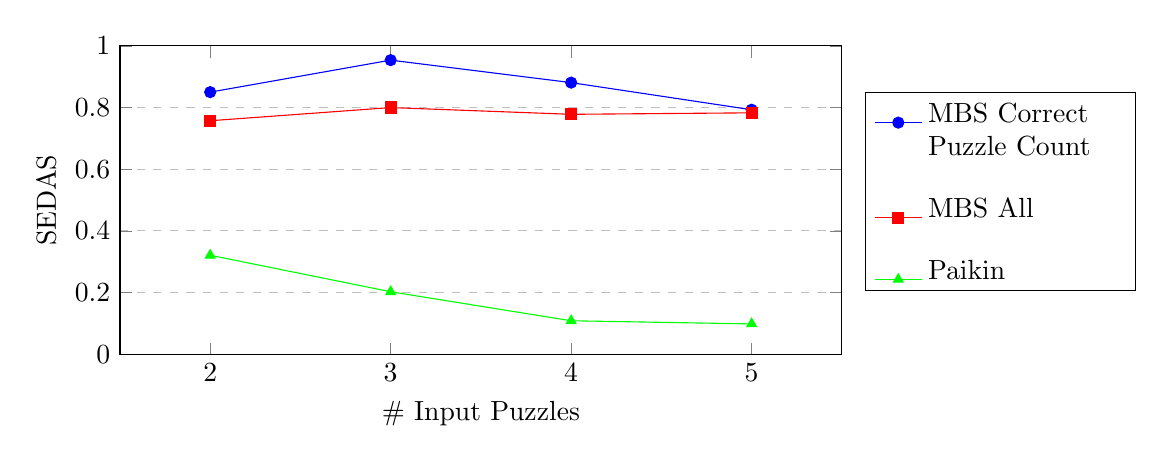
\begin{tikzpicture}
  \begin{axis}[
    height=5.5cm, width=10.75cm,
    xlabel={\# Input Puzzles},
    ylabel={SEDAS},
    xmin=1.5, xmax=5.5,
    ymin=0, ymax=1,
    xtick={2, 3, 4, 5},
    ytick={0,0.2,0.4,0.6,0.8,1.0},
    legend pos=north west,
    ymajorgrids=true,
    grid style=dashed,
    legend columns=1,
	legend style={at={(1.22,.85)},anchor=north,legend columns=-1,row sep=0.4cm,/tikz/nodes={text width=70pt,text depth=,anchor=base}},
    ]
\addplot [color=blue,mark=*,mark options={fill=blue}]
	coordinates {(2,0.849835) (3,0.953583)
		 (4,0.88068) (5,0.792796)};
\addplot [color=red,mark=square*,mark options={fill=red}]
	coordinates {(2,0.757159) (3,0.799822)
		 (4,0.777987) (5,0.782815)};
\addplot [color=green,mark=triangle*,mark options={fill=green}]
	coordinates {(2,0.321232) (3,0.202879)
		 (4,0.108857) (5,0.09866)};
\legend{MBS Correct Puzzle Count, MBS All, Paikin}
\end{axis}
\end{tikzpicture}\\
	(a) Shiftable Enhanced Direct Accuracy Score (SEDAS) \\~\\
	
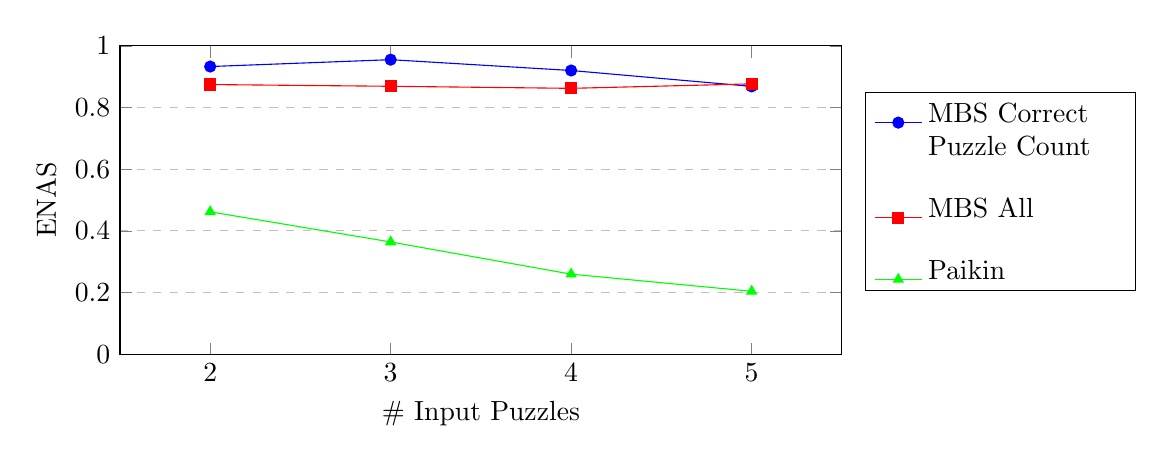
\begin{tikzpicture}
  \begin{axis}[
    height=5.5cm, width=10.75cm,
    xlabel={\# Input Puzzles},
    ylabel={ENAS},
    xmin=1.5, xmax=5.5,
    ymin=0, ymax=1,
    xtick={2, 3, 4, 5},
    ytick={0,0.2,0.4,0.6,0.8,1.0},
    legend pos=north west,
    ymajorgrids=true,
    grid style=dashed,
    legend columns=1,
	legend style={at={(1.22,.85)},anchor=north,legend columns=-1,row sep=0.4cm,/tikz/nodes={text width=70pt,text depth=,anchor=base}},
    ]
\addplot [color=blue,mark=*,mark options={fill=blue}]
	coordinates {(2,0.932805) (3,0.955051)
		 (4,0.919987) (5,0.868454)};
\addplot [color=red,mark=square*,mark options={fill=red}]
	coordinates {(2,0.874472) (3,0.868832)
		 (4,0.862183) (5,0.876654)};
\addplot [color=green,mark=triangle*,mark options={fill=green}]
	coordinates {(2,0.462006) (3,0.364242)
		 (4,0.259996) (5,0.204337)};
\legend{MBS Correct Puzzle Count, MBS All, Paikin}
\end{axis}
\end{tikzpicture}\\	
	
	(b) Enhanced Neighbor Accuracy Score (ENAS) \\~\\

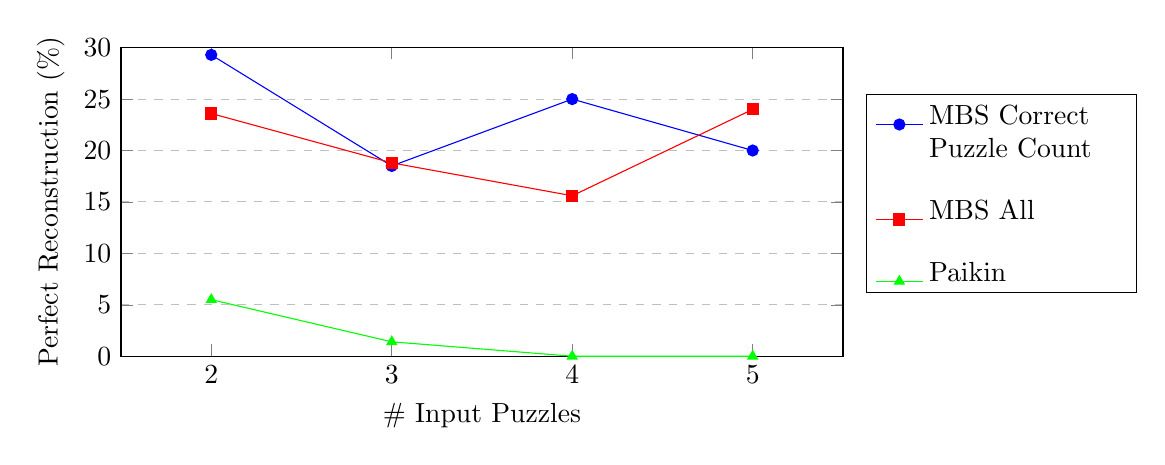
\begin{tikzpicture}
  \begin{axis}[
    height=5.5cm, width=10.75cm,
    xlabel={\# Input Puzzles},
    ylabel={Perfect Reconstruction (\%)},
    xmin=1.5, xmax=5.5,
    ymin=0, ymax=30,
    xtick={2, 3, 4, 5},
    ytick={0,5,10,15,20,25,30},
    legend pos=north west,
    ymajorgrids=true,
    grid style=dashed,
    legend columns=1,
	legend style={at={(1.22,.85)},anchor=north,legend columns=-1,row sep=0.4cm,/tikz/nodes={text width=70pt,text depth=,anchor=base}},
    ]
\addplot [color=blue,mark=*,mark options={fill=blue}]
	coordinates {(2,29.3) (3,18.5)
		 (4,25.0) (5,20.0)};
\addplot [color=red,mark=square*,mark options={fill=red}]
	coordinates {(2,23.6) (3,18.8)
		 (4,15.6) (5,24.0)};
\addplot [color=green,mark=triangle*,mark options={fill=green}]
	coordinates {(2,5.5) (3,1.4)
		 (4,0) (5,0)};
\legend{MBS Correct Puzzle Count, MBS All, Paikin}
\end{axis}
\end{tikzpicture}\\		
	
	(c) Percentage of Puzzles Perfectly Reconstructed \\

\end{tabular}
\caption{Performance of the Mixed-Bag and Paikin~\& Tal Solvers with Multiple Input Puzzles}\label{fig:graphSolverPerformanceComparison}
\end{figure}


As mentioned at the beginning of this chapter, images were randomly selected from the Pomeranz~\textit{et al.} dataset and provided to the Mixed-Bag Solver as well as Paikin~\& Tal's algorithm.  Table~\ref{tab:tableSolverPerformanceComparison} and Figure~\ref{fig:graphSolverPerformanceComparison} show the quantified quality of the outputs generated by  both solvers for varying input puzzle counts.   The three metrics used are the Shiftable Enhanced Direct Accuracy Score (SEDAS), Enhanced Neighbor Accuracy Score (ENAS), and the percentage of puzzles assembled perfectly (i.e., input and output puzzles are an identical match).  Note that the mean values of SEDAS and ENAS are displayed in the table and graphs; these means will calculated for all images that among the specified subset of solutions.  What is more, the results for the Mixed-Bag Solver (MBS) are subdivided between the case when the number of input puzzles was correctly determined (denoted with a ``$\dagger$'' in the table heading) versus all solver results (denoted with a ``$\ddagger$'').  This distinction is made since the solver accuracy when correctly identifying the number input puzzles represents the performance ceiling if the hierarchical clustering were optimal.

Across all quality metrics and categories, the Mixed-Bag Solver significantly outperformed Paikin~\& Tal' algorithm.  This is despite the fact that only Paikin~\& Tal's algorithm was provided additional information concerning the number of input puzzles.  What is more, unlike Paikin~\& Tal's algorithm, the Mixed Bag Solver saw no significant decrease in solver quality as the number of input puzzles were increased.  In addition, the Mixed-Bag Solver did not see a substantial difference in solution quality if it incorrectly estimated the number of input images; this indicates that these extra puzzles were relatively insignificant in size since they did not meaningfully affect SEDAS or ENAS.  

\section{Ten Puzzle Solving}

Paikin~\& Tal's~\cite{paikin2015} algorithm was shown to be able to solve up to five images simultaneously, which represents the most in the current literature.  To achieve this, their solver needed to be supplied with the number of input puzzles.  In contrast, this Mixed-Bag Solver has been shown to be able to solve up to ten puzzles of varying size.  Appendix~\ref{chap:tenPuzzleSolving} shows the input puzzles as well as the Mixed-Bag Solver's outputs. When the identical set of puzzles were supplied to Paikin~\& Tal's algorithm, the seeds for nine of the puzzles came from just three of the input puzzles.  

Table~\ref{tab:pomeranzBestBuddiesVisualizations} shows a comparison of the results between this thesis' Mixed-Bag Solver (MBS) and Paikin~\& Tal's algorithm's.  Despite the Mixed-Bag Solver receiving less information, it significantly outperformed Paikin~\& Tal receiving greater than 90\% accuracy for both  Shiftable Enhanced Direct Accuracy Score (SEDAS), and the Enhanced Neighbor Accuracy Score (ENAS) on all puzzles.  In contrast, Paikin~\& Tal only exceeded 90\% SEDAS and ENAS for image~(f). 

With respect to the unshifted, Enhanced Direct Accuracy Score (EDAS) metric, only four of the Mixed-Bag's solver outputs showed a shift that would affect EDAS while 7 of Paikin~\& Tal's outputs were shifted. This indicates that the Mixed-Bag Solver has a much greater immunity to shifts than Paikin~\& Tal's algorithm.

\begin{table}[tb]
\begin{center}
\begin{tabular}{ c|c||c|c||c|c||c|c } 
 \toprule
 \multicolumn{2}{c||}{Image} & \multicolumn{2}{c||}{Shifted} & \multicolumn{2}{c||}{SEDAS} & \multicolumn{2}{c}{ENAS} \\
\hline
 ID  & \# Pieces & MBS & Paikin & MBS & Paikin & MBS & Paikin  \\ 
\hline \hline
 (a) &  264     & No  & Yes & 1.000  & 0.000 & 1.000 & 0.544 \\ 
\hline
 (b) &  330     & No  & Yes & 1.000  & 0.000 & 1.000 &  0.090 \\ 
\hline
 (c) &  432     & Yes & Yes & 0.905 &  0.000 & 0.911 & 0.034 \\  
\hline
 (d) &  540     & No  & No  & 0.978 & 0.526 & 0.975 & 0.509 \\ 
\hline
 (e) &  540     & No  & No  & 1.000  &  0.059 & 1.000  & 0.327 \\ 
\hline
 (f) &  540     & Yes & No  & 0.978 & 0.943 & 0.917 & 0.931 \\ 
\hline
 (g) &  805     & No  & Yes & 0.997 &  0.000 & 0.990 &  0.077 \\ 
\hline
 (h) &  805     & Yes & Yes & 0.958 &  0.000   & 0.967 &  0.070 \\ 
\hline
 (i) &  805     & No  & Yes & 1.000  &  0.000   & 1.000  &  0.311 \\ 
\hline
 (j) &  805     & Yes & Yes & 0.998 &  0.000   & 0.990 &   0.073 \\ 
 \bottomrule
\end{tabular}
\end{center}
\caption{Comparison of the Image Shifting, SEDAS, and ENAS Results for the 10 Puzzle Dataset}\label{tab:pomeranzBestBuddiesVisualizations}
\end{table}